% SVN info for this file
\svnidlong
{$HeadURL$}
{$LastChangedDate$}
{$LastChangedRevision$}
{$LastChangedBy$}

\chapter{Proprietà varie ed eventuali}
\labelAppendix{proprietà}

\begin{introduction}
‘‘La Matematica consiste di fatti veri riguardanti oggetti immaginari.''
\begin{flushright}
	\textsc{Philip Davis e Reuben Hersh,} matematici immaginari con opinioni vere.
\end{flushright}
\end{introduction}

Riportiamo alcune proprietà utili per il lettore.
\section{Immagine e controimmagine}
Data una funzione $\funz{f}{X}{Y}$, per ogni sottoinsieme $A\subseteq X$ e $B\subseteq Y$ valgono le seguenti proprietà:
\begin{center}
	\begin{tabular}{l|l}
	\multicolumn{1}{c|}{\textbf{Immagine}} 	& \multicolumn{1}{c}{\textbf{Controimmagine}}\\ \hline
	$f(X)\subseteq Y$				& $f^{-1}(Y) = X$ 	\\ 
	$f(f^{-1}(Y)) = f(X)$			& $f^{-1}(f(X))= X$ \\
	$f(f^{-1}(B)) \subseteq B$ \footnotemark{}	& $f^{-1}(f(A)) \supseteq A$ \footnotemark{}	\\
	$f(f^{-1}(B)) = B \cap f(X)$	& $(f \mid_A)^{-1}(B) = A \cap f^{-1}(B)$											\\
	$f(f^{-1}(f(A))) = f(A)$		& $f^{-1}(f(f^{-1}(B))) = f^{-1}(B)$											\\
	$f(A) = \emptyset \iff A = \emptyset$	&  $f^{-1}(B) = \emptyset \iff B \subseteq Y \setminus f(X)$					\\
	$f(A) \supseteq B \iff \exists C \subseteq A \colon f(C) = B$ & $f^{-1}(B) \supseteq A \iff f(A) \subseteq B$\\
	$f(A) \supseteq f(X \setminus A) \iff f(A) = f(X)$ & $f^{-1}(B) \supseteq f^{-1}(Y \setminus B) \iff f^{-1}(B) = X$\\
	$f(X \setminus A) \supseteq f(X) \setminus f(A)$ & $f^{-1}(Y \setminus B) = X \setminus f^{-1}(B)$ \\
	$f(A \cup f^{-1}(B)) \subseteq f(A) \cup B$ & $f^{-1}(f(A) \cup B) \supseteq A \cup f^{-1}(B)$ \\
	$f(A \cap f^{-1}(B)) = f(A) \cap B$ & $f^{-1}(f(A) \cap B) \supseteq A \cap f^{-1}(B)$ \\
	\multicolumn{2}{c}{$f(A) \cap B = \emptyset \iff A \cap f^{-1}(B) = \emptyset$}
\end{tabular}
\addtocounter{footnote}{-2}
\stepcounter{footnote}\footnotetext{Uguale se $B\subseteq f(X)$, cioè se $f$ \textit{suriettiva}.}
\stepcounter{footnote}\footnotetext{Uguale se $f$ \textit{iniettiva}.}	
\end{center}

Date le funzioni $\funz{f}{X}{Y}$ e $\funz{f}{Y}{Z}$, valgono le seguenti proprietà:
\begin{itemize}
	\item $(g \circ f)(A) = g(f(A))$
	\item $(g \circ f)^{-1}(C) = f^{-1}(g^{-1}(C))$
\end{itemize}
Data una funzione $\funz{f}{X}{Y}$ e dati i sottoinsiemi $A_1,\ A_2\subseteq X$ e $B_1,\ B_2\subseteq Y$ valgono le seguenti proprietà:
\begin{center}
	\begin{tabular}{l|l}
		\multicolumn{1}{c|}{\textbf{Immagine}} 	& \multicolumn{1}{c}{\textbf{Controimmagine}}\\ \hline
		$A_1 \subseteq A_2 \implies f(A_1) \subseteq f(A_2)$	& $B_1 \subseteq B_2 \implies f^{-1}(B_1) \subseteq f^{-1}(B_2)$ 	\\ 
		$f(A_1 \cup A_2) = f(A_1) \cup f(A_2)$	& $f^{-1}(B_1 \cup B_2) = f^{-1}(B_1) \cup f^{-1}(B_2)$ \\
		$f(A_1 \cap A_2) \subseteq f(A_1) \cap f(A_2)$ \footnotemark{}	& $f^{-1}(B_1 \cap B_2) = f^{-1}(B_1) \cap f^{-1}(B_2)$	\\
		$f(A_1 \setminus A_2) \supseteq f(A_1) \setminus f(A_2)$  \footnotemark{} & $f^{-1}(B_1 \setminus B_2) = f^{-1}(B_1) \setminus f^{-1}(B_2)$
	\end{tabular}
\addtocounter{footnote}{-2}
\stepcounter{footnote}\footnotetext{\label{note1}Uguale se $f$ \textit{iniettiva}.}
\stepcounter{footnote}\footnotetext{Si veda \ref{note1}.}
\end{center}
Data una funzione $\funz{f}{X}{Y}$ e date le famiglie di sottoinsiemi $\{A_i\}\subseteq\setpart{X}$ e $\{B_i\}\subseteq\setpart{Y}$ (con $I$ un insieme di indici anche \textit{infinito} o \textit{non numerabile}) valgono le seguenti proprietà:
\begin{center}
	\begin{tabular}{l|l}
		\multicolumn{1}{c|}{\textbf{Immagine}} 	& \multicolumn{1}{c}{\textbf{Controimmagine}}\\ \hline
		$\displaystyle f\left(\bigcup_{i\in I}A_i\right) = \bigcup_{i\in I} f(A_i)$	& $\displaystyle f^{-1}\left(\bigcup_{i\in I}B_i\right) = \bigcup_{i\in I} f^{-1}(B_i)$ 	\\ 
		$\displaystyle f\left(\bigcap_{i\in I}A_i\right) \subseteq \bigcap_{i\in I} f(A_i)$ \footnotemark{}	& $\displaystyle f^{-1}\left(\bigcap_{i\in I}B_i\right) = \bigcap_{i\in I} f^{-1}(B_i)$
	\end{tabular}
\addtocounter{footnote}{-1}
\stepcounter{footnote}\footnotetext{Si veda \ref{note1}.}
\end{center}
	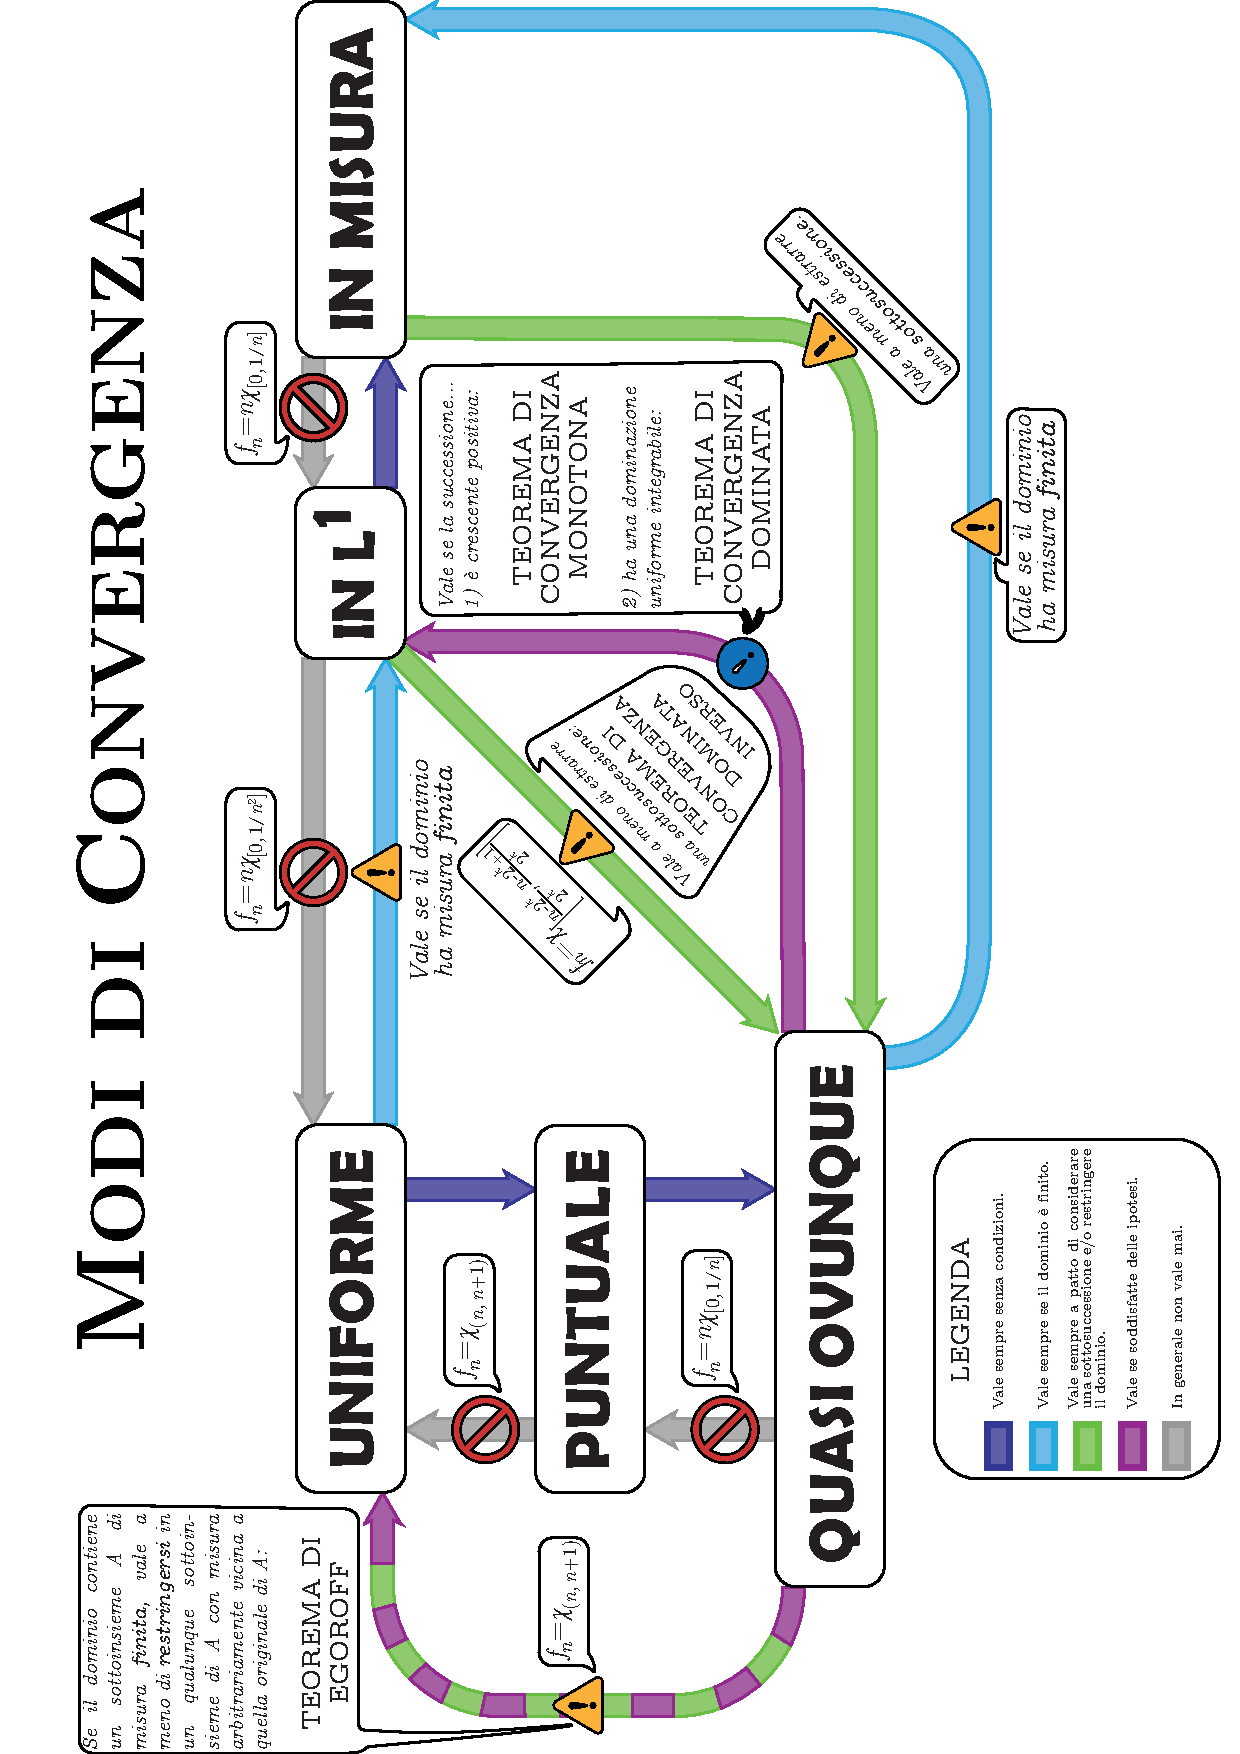
\includepdf{images/modiconvergenza2}
\newpage
\section{Passaggio al limite sotto segno di integrale}
	\begin{tabular}{p{0.49\textwidth}p{0.49\textwidth}}
		\multicolumn{2}{c}{\textbf{TEOREMA}} \\
		\begin{tabular}[c]{m{0.49\textwidth}}
		\centering \textbf{Convergenza uniforme} \\ \centering \textbf{(teoria di Riemann)}
		\end{tabular} &
		\begin{tabular}[c]{m{0.49\textwidth}}
		\centering \textbf{Convergenza uniforme} \\ \centering \textbf{(teoria di Lebesgue)}
		\end{tabular} \\
		Siano $\funz{f_n,f}{\left[a,b\right]}{\realset},\ n\geq 1$ tali che	\begin{enumerate}[label=(\alph*)]
			\item $f_n\in\mathcal{R}\left(\left[a,b\right]\right),\ \forall n\geq 1$.
			\item $f_n$ converge uniformemente a $f$ su $\left[a,b\right]$.
		\end{enumerate}
		Allora
		\begin{enumerate}
			\item $f\in\mathcal{R}\left(\left[a,b\right]\right)$.
			\item 
			Vale il \textbf{passaggio al limite sotto segno di integrale}:
			\begin{tabular}[c]{c}
			$\displaystyle\lim_{n\to+\infty}\int_{a}^{b}\!\!\! f_n(x)dx=\int_{a}^{b}\!\!\!\lim_{n\to+\infty}f_n(x)dx$
			\end{tabular}
		\end{enumerate} &
		Consideriamo lo spazio di misura $\left(X,\mathcal{M},\mu\right)$ e le funzioni $\funz{f_n,f}{X}{\complexset}$ tali che
		\begin{enumerate}[label=(\alph*)]
			\item $f_n\in L^{1}\left(\mu\right)$.
			\item $f_n$ converge uniformemente a $f$ su $X$.
			\item $\mu(X)<+\infty$.
		\end{enumerate}
			Allora
		\begin{enumerate}
			\item $f\in L^{1}\left(\mu\right)$.
			\item $\displaystyle\lim_{n\to+\infty}\norm{f_n-f}_1=0$.
			\item Vale il \textbf{passaggio al limite sotto segno di integrale}:
			\begin{tabular}[c]{c}
			$\displaystyle\lim_{n\to+\infty}\int_X\!\!\! f_nd\mu=\int_X\!\!\lim_{n\to+\infty}f_nd\mu$
			\end{tabular}
		\end{enumerate} \\
		\multicolumn{2}{c}{\textbf{VANTAGGI}} \\
		\begin{itemize}
			\item È l'unico teorema di questo tipo valido nella teoria di Riemann.
		\end{itemize} &
		\begin{itemize}
			\item Vale su spazi di misura finita invece che solamente degli intervalli finiti.
		\end{itemize} \\
		\multicolumn{2}{c}{\textbf{SVANTAGGI}} \\
		\begin{itemize}
			\item Richiede la convergenza uniforme.
			\item Vale solo per funzioni limitate.
			\item Vale solo su intervalli limitati.
		\end{itemize} &
		\begin{itemize}
			\item Richiede la convergenza uniforme.
			\item Richiede l'integrabilità della successione.
			\item Vale solo su spazi di misura finita.
		\end{itemize}
		\begin{comment} \\
		\multicolumn{1}{l}{
			\begin{tabular}[c]{p{3cm}}
				Siano $\funz{f_n,f}{\left[a,b\right]}{\realset},\ n\geq 1$ tali che	\begin{enumerate}
					\item $f_n\in\mathcal{R}\left(\left[a,b\right]\right),\ \forall n\geq 1$.
					\item $f_n$ converge uniformemente a $f$ su $\left[a,b\right]$.
				\end{enumerate}
				Allora
				\begin{enumerate}
					\item $f\in\mathcal{R}\left(\left[a,b\right]\right)$.
					\item Vale il \textbf{passaggio al limite sotto segno di integrale}:\\
					$\displaystyle	\lim_{n\to+\infty}\int_{a}^{b}f_n(x)dx=\int_{a}^{b}\lim_{n\to+\infty}f_n(x)dx=\int_{a}^{b}f(x)dx$
				\end{enumerate}
		\end{tabular}} &
		\multicolumn{1}{l}{
			\begin{tabular}[c]{p{3cm}}
				Siano $\left(X,\mathcal{M},\mu\right)$ uno spazio di misura e $\funz{f_n,f}{X}{\left[0,+\infty\right]}$ con $n\geq 1$ tali che	\begin{enumerate}
					\item $f_n$ sono misurabili.
					\item $\displaystyle\lim_{n\to+\infty}f_n(x)=f(x),\ \forall x\in X$.
					\item $0\leq f_n(x)\leq f_{n+1}(x),\ \forall n\geq 1,\ \forall x\in X$.
				\end{enumerate}
				allora
				\begin{enumerate}
					\item $f$ è misurabile.
					\item Vale il \textbf{passaggio al limite sotto segno di integrale}:\\
					$\displaystyle	\lim_{n\to+\infty}\int_Xf_nd\mu=\int_Xfd\mu\in\left[0,+\infty\right]$
				\end{enumerate}
		\end{tabular}}&
		\begin{tabular}[c]{p{3cm}}
			Sia $\left(X,\mathcal{M},\mu\right)$ uno spazio di misura e $\funz{f_n}{X}{\complexset}$ una successione di funzioni misurabili tale che esiste\\
			$\displaystyle f(x)=\lim_{n\to+\infty}f_n(x),\ \forall x\in X$
			Se esiste una funzione $g\in \mathcal{L}^{1}\left(\mu\right)$ tale per cui\\
			$\displaystyle\abs{f_n(x)}\leq g(x),\ \forall n\geq 1,\ \forall x\in X$
			allora $f\in \mathcal{L}^{1}\left(\mu\right)$ e vale\\
			$\displaystyle \lim_{n\to+\infty}\int_X\abs{f_n-f}d\mu=0$
			e vale il \textbf{passaggio al limite sotto segno di integrale}:
			$\displaystyle \lim_{n\to+\infty}\int_Xf_nd\mu=\int_Xfd\mu$
		\end{tabular} &
		\begin{tabular}[c]{@{}l@{}}
			Consideriamo lo spazio di misura $\left(X,\mathcal{M},\mu\right)$ e le funzioni $\funz{f_n,f}{X}{\complexset}$. Se
			\begin{enumerate}[label=(\alph*)]
				\item $f_n\in L^{1}\left(\mu\right)$.
				\item $f_n$ converge uniformemente a $f$ su $X$.
				\item $\mu(X)<+\infty$.
			\end{enumerate}
			allora
			\begin{enumerate}
				\item $f\in L^{1}\left(\mu\right)$.
				\item $\displaystyle\lim_{n\to+\infty}\norm{f_n-f}_1=0$.
				\item Vale il \textbf{passaggio al limite sotto segno di integrale}\\
				$\displaystyle \lim_{n\to+\infty}\int_Xf_nd\mu=\int_Xfd\mu$
			\end{enumerate}
		\end{tabular} \\
		\multicolumn{4}{c}{\textbf{VANTAGGI}} \\
		\multicolumn{1}{l}{
			\begin{tabular}[c]{p{3cm}}
				\begin{enumerate}
					\item È l'unico teorema di questo tipo valido nella teoria di Riemann.
				\end{enumerate}
		\end{tabular}} &
		\begin{tabular}[c]{p{3cm}}
			\begin{enumerate}
				\item Richiede la convergenza puntuale.
				\item Si può applicare anche con la convergenza \textbf{q.o.} purché la misura sia completa o la funzione limite $f$ è una funzione misurabile che coincide \textbf{q.o.} con il limite \textbf{q.o.} della successione.
				\item È sufficiente anche solamente supporre che la successione $f_n$ sia non decrescente su $X$ \textbf{q.o.}.
				\item Vale qualunque sia la misura di $X$.
			\end{enumerate}
		\end{tabular} &
		\begin{tabular}[c]{p{3cm}}
			\begin{enumerate}
				\item Richiede la convergenza puntuale.
				\item Si può applicare anche con la convergenza \textbf{q.o.} e con la dominazione \textbf{q.o.} purché la misura sia completa o la funzione limite $f$ è una funzione misurabile che coincide \textbf{q.o.} con il limite \textbf{q.o.} della successione.
				\item Vale qualunque sia la misura di $X$.
				\item Vale per funzione a valori complessi.
			\end{enumerate}
		\end{tabular} &
		\begin{tabular}[c]{@{}l@{}}
			\begin{enumerate}
				\item Vale su spazi di misura finita invece che solamente degli intervalli finiti.
			\end{enumerate}
		\end{tabular} \\
		\multicolumn{4}{c}{\textit{\textbf{SVANTAGGI}}} \\
		\multicolumn{1}{l}{
			\begin{tabular}[c]{@{}l@{}}
				\begin{enumerate}
					\item Richiede la convergenza uniforme.
					\item Vale solo per funzioni limitate.
					\item Vale solo su intervalli limitati.
				\end{enumerate}
		\end{tabular}} &
		\begin{tabular}[c]{@{}l@{}}
			\begin{enumerate}
				\item Non vale per successioni decrescenti.
			\end{enumerate}
		\end{tabular} &
		\begin{tabular}[c]{@{}l@{}}
			\begin{enumerate}
				\item Richiede una dominazione della successione. \end{enumerate}
		\end{tabular} &
		\begin{tabular}[c]{@{}l@{}}
			\begin{enumerate}
				\item Richiede la convergenza uniforme.
				\item Richiede l'integrabilità della successione.
				\item Vale solo su spazi di misura finita.
			\end{enumerate}
		\end{tabular}
	\end{comment}
	\end{tabular}